\documentclass[a4paper, bibgerm]{article}
\usepackage[utf8]{inputenc}
\usepackage[T1]{fontenc}
\usepackage{lmodern}
\usepackage{ngerman}
\usepackage{bibgerm}
\usepackage{color}
\usepackage{amssymb,amsmath}
\usepackage{graphicx}
\usepackage{subfig}
\usepackage{hyperref}
\usepackage{listings}

\lstloadlanguages{Haskell}
\lstnewenvironment{code}
  {\lstset{}%
    \csname lst@SetFirstLabel\endcsname}
  {\csname lst@SaveFirstLabel\endcsname}
\lstset{
  basicstyle=\small\ttfamily,
  flexiblecolumns=false,
  basewidth={0.5em,0.45em},
  literate={+}{{$+$}}1 {/}{{$/$}}1 {*}{{$*$}}1 {=}{{$=$}}1
  {>}{{$>$}}1 {<}{{$<$}}1 {\\}{{$\lambda$}}1
  {\\\\}{{\char`\\\char`\\}}1
  {->}{{$\rightarrow$}}2 {>=}{{$\geq$}}2 {<-}{{$\leftarrow$}}2
  {<=}{{$\leq$}}2 {=>}{{$\Rightarrow$}}2 
  {.}{{$\circ$}}2
% {\ .\ }{{$\circ$}}2
  {>>>}{{$\ggg$}}2
%  {>>}{{>>}}2 {>>=}{{>>=}}2 %<<
  {|}{{$\mid$}}1               
}

\newcommand{\defaultscale}{0.3}

\newcommand\lsection{}
\newcommand\lsubsection{}
\newcommand\lsubsubsection{}
\newcommand\lparagraph{}
\newcommand\sref{}
\newcommand\abb{}
\newcommand\fig{}
\newcommand\figs{}
\newcommand\subfig{}
\newcommand\vertfig{}
\newcommand\clipvertfig{}

\newcommand{\project}[1]{%
  \renewcommand\lsection[2][\LSectionDefault]{%
    \def\LSectionDefault{##2}%
    \section{##2}
    \label{#1:sec:##1}%
  }
  \renewcommand\lsubsection[2][\LSubSectionDefault]{%
    \def\LSubSectionDefault{##2}%
    \subsection{##2}
    \label{#1:sec:##1}%
  }
  \renewcommand\lsubsubsection[2][\LSubSubSectionDefault]{%
    \def\LSubSubSectionDefault{##2}%
    \subsubsection{##2}
    \label{#1:sec:##1}%
  }
  \renewcommand\lparagraph[2][\LParagraphDefault]{%
    \def\LParagraphDefault{##2}%
    \paragraph{##2}
    \label{#1:sec:##1}%
  }  
  \renewcommand\sref[1]{%
    Abschnitt~\ref{#1:sec:##1}
  }%
  \renewcommand{\abb}[1]{Abb.\ref{#1:fig:##1}}
  \renewcommand{\fig}[3][\defaultscale]{%
    \begin{figure}[htp]
      \centering
      \includegraphics[scale=##1]{images/##2}
      \caption{##3}
      \label{#1:fig:##2}
  \end{figure}}

  \renewcommand{\figs}[3]{%
    \begin{figure}[htp]
      \centering
      ##3
      \caption{##2}
      \label{#1:fig:##1}
    \end{figure}
  }

  \renewcommand{\subfig}[3][\defaultscale]{%
    \subfloat[##3]{
      \includegraphics[scale=##1]{images/##2}
      \label{#1:fig:##2}
    }
  }

  \renewcommand{\vertfig}[3][\defaultscale]{%
    \begin{sidewaysfigure}[htp]
      \centering
      \includegraphics[scale=##1]{images/##2}
      \caption{##3}
      \label{#1:fig:##2}
    \end{sidewaysfigure}%
  }

  \renewcommand{\clipvertfig}[5]{%
    \begin{sidewaysfigure}[htp]
      \centering
      \includegraphics*[scale=##1, viewport=##2]{images/##3}
      \caption{##5}
      \label{#1:fig:##4}
    \end{sidewaysfigure}%
  }
}

\project{magicl}

\newcommand\icode[1]{\lstinline?#1?}
\newcommand\ato{\rightarrow}

\newtheorem{defini}{Definition}

\newcommand{\defi}[2]{%
  \begin{defini}[#1]
    \label{def:#1}
    #2
  \end{defini}
}

\newcommand{\dref}[1]{Def. \ref{def:#1}}

\begin{document}

\title{MagicL: Ein Arrow-basiertes Compilerbau-Framework}
\author{Benjamin Teuber}
\date{\today}

% \maketitle

\begin{abstract}
  MagicL ist der Prototyp eines universellen Frameworks für den Entwurf
  von Programmier- und Auszeichnungssprachen. Es soll dem
  Meta-Programmierer praktische Werkzeuge für das Parsing und Übersetzen
  neuer sowie für Generation von Code bestehender Sprachen an die Hand
  geben, wobei insbesondere (jedoch nicht ausschließlich) aus
  S-Expressions aufgebaute Sprachen unterstützt werden. Die Parser- und
  Compilererstellung erfolgt nach einem kategorientheoretisch
  motivierten Baukastenansatz, so dass beispielsweise Parser durch die
  Kombination von Arrows erzeugt werden.
\end{abstract}

% \tableofcontents

\section{Einleitung}
\label{sec:intro}

Modellgetriebene Softwareentwicklung ist in aller Munde: Während UML
bald sein 20-Jähriges Jubiläum \footnote{Zumindest was die ersten
  Entwürfe angeht - der Standardisierungsprozess war erst 1997
  abgeschlossen.} feiert, verspricht Microsoft mit \textit{Oslo}
\cite{TODO} einen ``Mainstream-Ansatz für Modellierung''. IBM vermarktet
seit Jahren \textit{Rational Application Developer}, das wie auch das
freie \textit{Eclipse Modelling Framework} oder auch \textit{Enterprise
  Architect} Eclipse um modellbasierte Codegenerierung bereichern.
Code-Generation fällt auch im World Wide Web eine immer größer werdende
Rolle zu: Ob \textit{Ruby on Rails} oder \textit{Google Web Toolkit},
praktisch alle Web Frameworks generieren zumindest ihre HTML-Dateien oder
SQL-Strings für den Datenbankzugriff.

Der ganze Bereich um Code-Generation ist also ein aktuelles Thema.

\subsection{Codegenerierung}
\label{sec:intro:codegen}

Allgemein ist jedermann klar, was Codegenerierung bedeutet:
Das automatisiertes Erzeugen von Quelltext. Dennoch gibt es diverse
Unterschiede zwischen Codegenerierungswerkzeugen.

So differenziert man zwischen aktiver und passiver
Codegenerierung. Aktiv bedeutet, dass die Generierung wiederholt
ausgeführt werden kann, wenn sich etwas am Modell oder Generator ändert,
da die komplette Datei generiert wird. Passiv generierter Code dagegen
wird anschließend vom Programmierer modifiziert bzw. erst mit sinnvollen
Inhalten bestückt, so dass dieser nur normalerweise nur einmalig
generiert werden kann, wenn die Anpassungen nicht überschrieben werden
sollen. Zwischen aktiver und passiver Generierung liegen Dateien, in
denen nur markierte Abschnitte generiert werden - so dass der Rest
unverändert bleiben kann. Optimal wäre natürlich ein allgemeiner
Merge-Mechanismus, der die Arbeit des Programmierers reibungslos in die
neue Version übernimmt - dies ist aber leider schwierig zu
implementieren.

Zudem lässt sich nach Ein- und Ausgabe des Generators unterscheiden.

Vorteile:
\begin{itemize}
\item Abstraktion - Modellarchitekten beötigen keine
  Programmiersprachkenntnisse, Backend austauschbar
``Ist die Sprache an die Problemdomäne angepasst, muss man das Problem
nicht in die Sprache zwängen''
\item Produktivität - DRY-Prinzip spart u.U. viel Zeit
\item Qualität - ist der Generator fehlerfrei, gibt es keine Probleme
  bei neuen Modellen
\item Konsistenz - einheitliche Strukturen/Namen, minimiert Einarbeitungszeit
\end{itemize}

Nachteile:
\begin{itemize}
\item Dokumentation / Einarbeitung
\item Fehlersuche
\item Komplexität
\item Entwicklungsaufwand
\end{itemize}

\subsection{Lisp}
\label{sec:into:lisp}

-Code-Generation und Metaprogrammierung seit fast 50 Jahren
-was können wir lernen?
--Einheitliche Syntax macht vieles leichter
--compilererweitungen durch makros

\subsubsection{Vergleich mit XML}
\label{sec:intro:lisp:xml}

-gleiche Zielsetzung - Baumstruktur
-syntax: ``</tag>'' vs. ``)''
--nur vorteilhaft f texteditor ohne parent-matching!
-XML komplexer, da Attribute
--kann auch durch unterknoten ausgedrückt werden - wird es nur aufgrund
von hässlicher syntax nicht
--nicht mehr rekursiv, komplexe attribute gehen nicht (wirklich)

diskussion: makros good or bad

\subsection{Zielsetzung}
\label{sec:intro:goal}

\section{Erster Prototyp in Ruby}
\label{sec:sexy}

\section{Arrow-basierte Implementation in Haskell}
\label{sec:magicl}

\subsection{Kategorientheoretische Grundlagen}
\label{sec:catbasics}

Die Kategorientheorie ist ein sehr abstrakter Zweig der Mathematik -
aber auch ein universeller, denn fast alle wichtigen mathematischen
Strukturen sind Kategorien. Kategorientheorie findet dank seiner
Allgemeinheit und Anwendbarkeit für Berechnungen auch in der Informatik
eine immer größer werdende Rolle. Die Implementation von MagicL benutzt
einige kategorientheorietische Begriffe , z.B. werden Parser als
zusammengesetzte Funktoren konstruiert. Dieser Abschnitt führt in die
Kategorientheorie ein und stellt alle später verwendeten Konzepte
vor. Die Definitionen sind weitgehend aus \cite{Grundlagen} übernommen.

\fig[0.3]{cat_funs}{Ein simples Funktionensystem}

Der Grundansatz der Kategorientheorie ist die Verallgemeinerung der
Art und Weise, wie mit Funktionstypen gerechnet wird - insbesondere
hinsichtlich der Komposition von Funktionen. \abb{cat_funs} zeigt ein
kleines Funktionensystem zwischen den Mengen $\mathbb{R} \times
\mathbb{R}$, $\mathbb{R}$ und $\mathbb{Z}$. Es kommen folgende
Funktionen vor:
\begin{itemize}
\item $+ : \mathbb{R} \times \mathbb{R} \ato \mathbb{R}$ addiert zwei
  reelle Zahlen.
\item $\mathrm{abs} : \mathbb{R} \ato \mathbb{Z}$ ist die Betragsfunktion.
\item $+1 : \mathbb{Z} \ato \mathbb{Z}$ addiert $1$ zu einer ganzen Zahl.
\item $\mathrm{abs} \circ + : \mathbb{R} \times \mathbb{R} \ato \mathbb{Z}$
  addiert zwei reelle Zahlen und bildet anschließend den Betrag.
\end{itemize}

Die Komposition $\mathrm{abs} \circ +$ (gesprochen "`abs \textit{nach} +"') lässt
sich bilden, weil der Definitionsbereich von $\mathrm{abs}$ mit dem
Zielbereich von $+$ übereinstimmt (nämlich $\mathbb{R}$). Es lassen sich
also zwei im Diagramm aufeinander folgende Pfeile zu einem direkten
zusammenfassen. Die Kategorientheorie "`vergisst"' nun den Bezug zu
Mengen und Funktionen und arbeitet statt dessen abstrakt mit Objekten
und Morphismen.

\defi{Kategorie}{
Eine Kategorie $\mathbf{C} = (\mathrm{Ob}^\mathbf{C}, \mathrm{Mor}^\mathbf{C},
\circ^\mathbf{C}, \mathrm{id}^\mathbf{C})$ ist gegeben durch 
\begin{itemize}
\item eine Klasse $\mathrm{Ob}^\mathbf{C}$ von Objekten\footnote{Da Objekte selbst Mengen
    sein können, wäre eine Definition von $\mathrm{Ob}^\mathbf{C}$ als Menge problematisch.}.
\item eine Menge Morphismen $\mathrm{Mor}^\mathbf{C}_{A,B}$ für alle $ A,B \in
  \mathrm{Ob}^\mathbf{C}$, wobei $A$ und $B$ Domäne und Codomäne genannt werden,
\item einen Kompositionsoperator $\circ^\mathbf{C}_{A,B,C}$ für alle $
  A,B,C \in \mathrm{Ob}^\mathbf{C}$ mit \\
  $\circ^\mathbf{C}_{A,B,C} : \mathrm{Mor}^\mathbf{C}_{B,C} \times
  \mathrm{Mor}^\mathbf{C}_{A,B} \rightarrow \mathrm{Mor}^\mathbf{C}_{A,C}$,
\item eine Identität $\mathrm{id}^\mathbf{C}_A \in \mathrm{Mor}^\mathbf{C}_{A,A}$ für alle $ A \in \mathrm{Ob}^\mathbf{C}$,
\end{itemize}
wobei folgende Axiome erfüllt sein müssen:
\begin{itemize}
\item Neutralität der Identität: $$f \circ_{A,A,B} \mathrm{id}_A = \mathrm{id}_B \circ_{A,B,B} f = f$$
\item Assoziativität:
  $$f \circ_{A,C,D} (g \circ_{A,B,C} h) = (f \circ_{B,C,D} g) \circ_{A,B,D}h$$
\end{itemize}
}

\fig{cat_comp}{Das Assoziativitätsaxiom als kommutatives Diagramm}

Indizes und Kategorien werden der Einfachheit halber weggelassen, wenn
sie aus dem Kontext hervorgehen. Viele Definitionen der
Kategorientheorie erfolgen über kommutative Diagramme:
\defi{Kommutatives Diagramm}{ Ein Diagramm kommutiert, wenn für je zwei
  eingezeichnete Pfade $f=f_1 \circ \cdots \circ f_n : A \rightarrow B$
  und $g=g_1 \circ \cdots \circ g_n : A \rightarrow B$ zwischen zwei
  Objekten $A$ und $B$ die Gleichung $f=g$ gilt.  } 
Beispielsweise zeigt \abb{cat_comp} das Assoziativitätsaxiom als
kommutatives Diagramm. $g$ ist nur der Vollständigkeit halber
eingezeichnet und spielt für das kommutative Diagramm selbst keine
Rolle. Dieses Diagramm dient lediglich der Veranschaulichung, ist aber
nicht selbst für die Definition der Assoziativität geeignet -
schließlich setzt \dref{Kommutatives Diagramm} bereits Assoziativität
von $\circ$ voraus. 

Wie das Einführungsbeispiel erwarten lässt, bilden die Mengen und
Funktionen eine Kategorie, genannt $\mathbf{Set}$. \abb{cat_simple} zeigt eine
andere simple Beispielkategorie, die aus den Objekten $A, B$ und den
Morphismen $f, g, \mathrm{id}_A, \mathrm{id}_B$ besteht. Alle Kompositionen
dieser Morphismen sind wieder in $\mathrm{Mor}^{\mathbf{Set}}$ - denn
jede Kategorie ist selbstverständlich unter Komposition geschlossen.

\fig[0.3]{cat_simple}{Eine einfache Kategorie}

Strukturerhaltende Abbildungen zwischen Kategorien werden Funktoren genannt:

\defi{Funktor}{
Ein Funktor $F=(F_{\mathrm{Ob}},F_{\mathrm{Mor}}) : \mathbf{C}
\rightarrow \mathbf{D}$ von Kategorie $C$ nach Kategorie $D$  
    \begin{itemize}
    \item bildet jedes Objekt $A \in \mathrm{Ob}^{\mathbf{C}}$ auf $F_{\mathrm{Ob}}(A) \in
      \mathrm{Ob}^{\mathbf{D}}$ ab, 
    \item bildet jeden Morphismus $f \in
      \mathrm{Mor}^{\mathbf{C}}_{A,B}$ auf $F_{\mathrm{Mor}}(f) \in
      \mathrm{Mor}^{\mathbf{D}}_{F_{\mathrm{Ob}}(A),F_{\mathrm{Ob}}(B)}$
      ab,
    \end{itemize}   
    wobei für alle $A,B,C \in \mathrm{Ob}^{\mathbf{C}}$ und alle $f \in
    \mathrm{Mor^{\mathbf{C}}_{B,C}},g \in
    \mathrm{Mor^{\mathbf{C}}_{A,B}}$ folgende Axiome erfüllt sein 
    müssen: 
    \begin{itemize}
    \item Erhaltung der Komposition:
      $$F_{\mathrm{Mor}}(f \circ^{\mathbf{C}} g) =
      F_{\mathrm{Mor}}(f) \circ^{\mathbf{D}} F_{\mathrm{Mor}}(g)$$
    \item Erhaltung der Identität:
      $$F_{\mathrm{Mor}}(\mathrm{id}^{\mathbf{C}}_A) =
      \mathrm{id}^{\mathbf{D}}_{F_{\mathrm{Ob}}(A)}$$
    \end{itemize}
}

Die Kategorientheorie schafft es, Begriffe für Funktionseigenschaften
wie Injektivität sowie Mengenoperationen wie das kartesische Produkt auf
Kategorien zu verallgemeinern, indem sich die neuen Definitionen
ausschließlich auf Objekte und Morphismen beziehen und nicht von Mengen
oder Funktionen im speziellen Gebrauch machen. In der Kategorie
$\mathbf{Set}$ stimmen die neuen Begriffe dann genau mit den alten
überein. Dem kartesischen Produkt entspricht das Produkt von Objekten:

\defi{Produkt}{
  Ein Objekt $A \times B$ mit zwei Projektionsmorphismen $\pi_1
  \in \mathrm{Mor}_{A \times B,A}$ und $\pi_2 \in \mathrm{Mor}_{A \times
    B,B}$ ist ein Produkt von $A$ und $B$, wenn für jedes $X \in
  \mathrm{Ob}$ und alle $f \in \mathrm{Mor}_{X,A},g \in
  \mathrm{Mor}_{X,B}$ genau ein Morphismus
  $\langle f,g \rangle \in \mathrm{Mor}_{X,A \times B}$ existiert, für den \abb{cat_product} kommutiert, d.h. 
  $\pi_1 \circ \langle f,g \rangle = f$ und $\pi_2 \circ \langle f,g \rangle = g$ gelten.
}

\begin{figure}
  \centering
  \subfloat[Produkt]{
    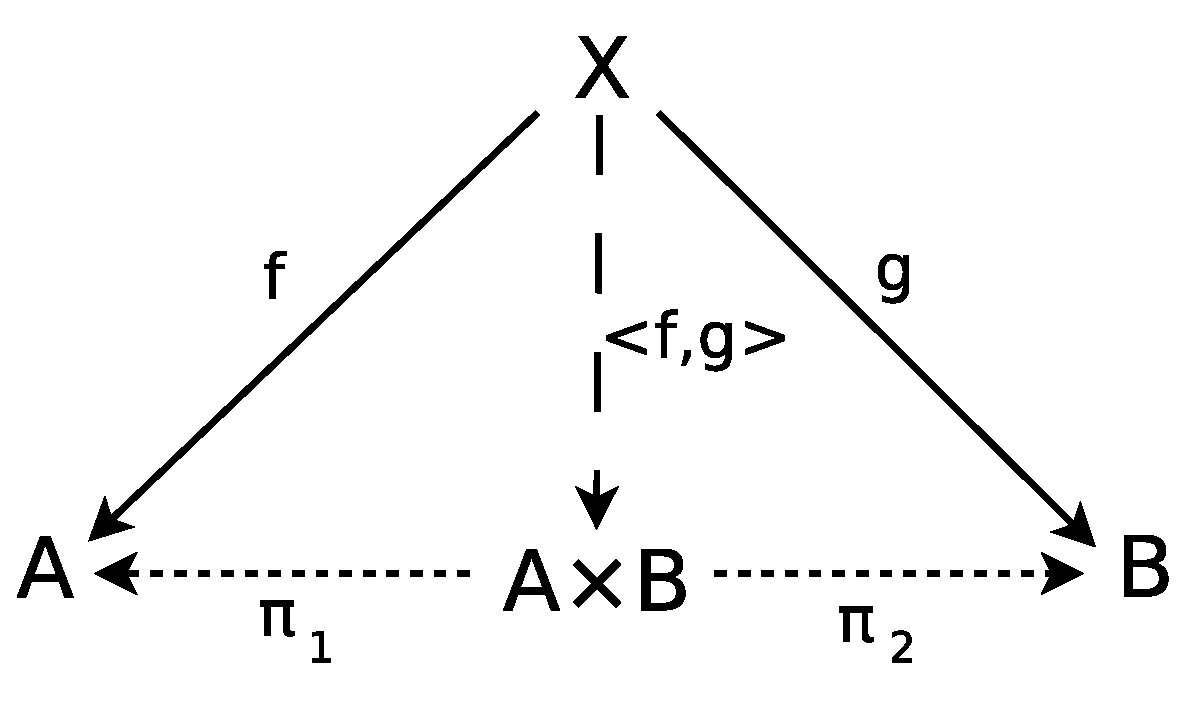
\includegraphics[scale=0.3]{images/cat_product}
    \label{magicl:fig:cat_product}
  }
  \subfloat[Coprodukt]{
    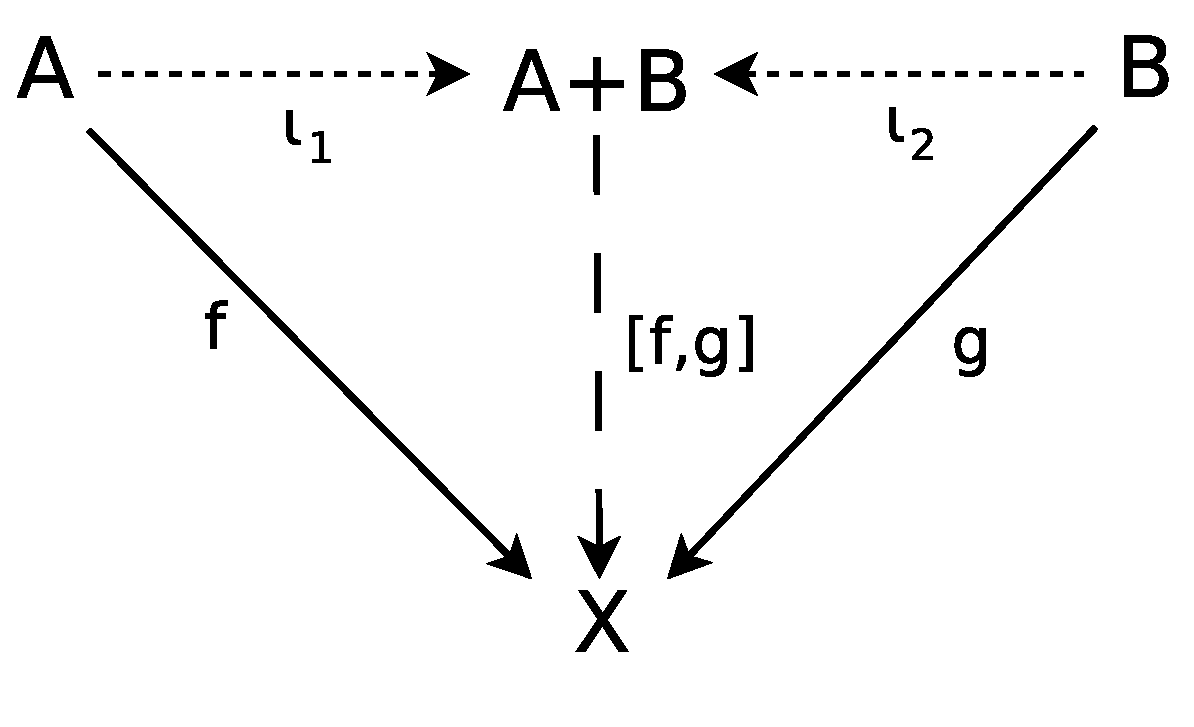
\includegraphics[scale=0.3]{images/cat_coproduct}
    \label{magicl:fig:cat_coproduct}
  }
  \caption{Kommutative Diagramme zur Definition von Produkt und Coprodukt}
\end{figure}

Man kann leicht nachvollziehen, dass das kartesische Produkt genau ein
Produkt für die Kategorie $\mathbf{Set}$ ist. $\langle f,g \rangle$ ist
hier die Funktion, die einem Tupel $(x,y)$ den Funktionswert $(f(x),
g(y))$ zuordnet.

Dreht man im Diagramm alle Pfeile um, erhält man die Definition für das
Coprodukt, ein zum Produkt dualer\footnote{Die zu einer Kategorie
  $\mathbf{C}$ duale Kategorie $\mathbf{C}^{\mathrm{op}}$ entsteht
  nämlich durch das Umdrehen von Pfeilen.} Operator:

\defi{Coprodukt}{
  Ein Objekt $A + B$ mit zwei Injektionsmorphismen $\iota_1
  \in \mathrm{Mor}_{A,A + B}$ und $\iota_2 \in \mathrm{Mor}_{B,A +
    B}$ ist ein Coprodukt von $A$ und $B$, wenn für jedes $X \in
  \mathrm{Ob}$ und alle $f \in \mathrm{Mor}_{A,X},g \in
  \mathrm{Mor}_{B,X}$ genau ein Morphismus
  $[f,g] \in \mathrm{Mor}_{A + B,X}$ existiert, für den \abb{cat_coproduct} kommutiert, d.h. 
  $[f,g] \circ \iota_1 = f$ und $[f,g] \circ \iota_2 = g$ gelten.
}

Das Coprodukt entspricht einer disjunkten Vereinigung von Mengen, also
einer Vereinigung von Mengen. die vorher explizit disjunkt gemacht
werden (sofern sie es nicht bereits sind). Dies kann beispielsweise durch
die Indizes $L$ und $R$ geschehen: $\{1,2,3\} + \{2,3,4\} =
\{1_L,2_L,3_L,2_R,3_R,4_R\}$. Der Morphismus $[f,g]$ entspricht einer
Fallunterscheidung: Auf Elemente aus $A$ wird $f$ angewendet, auf welche
aus $B$ entsprechend $g$.

(Optional: Natürliche Transformationen, Monaden, Kleisli-Kategorie)

\subsection{Kategorien in Haskell}
\label{sec:cats_haskell}

Die Haskell-Bibliotheken bieten viele kategorientheotische Begriffe an,
die allerdings immer bestimmten Einschränkungen
unterliegen. Beispielsweise sind die Objekte einer Kategorie hier immer
Haskell-Typen. Die Typklasse \icode{Category} ist wie folgt definiert:
\begin{code}
class Category cat where
  id   :: cat a a
  (.) :: cat b c -> cat a b -> cat a c
\end{code}
Ein Typ \icode{cat}, der selbst zwei Typparameter benötigt, ist also eine
Instanz von \icode{Category}, wenn es generische Identitäts- und
Kompositionsoperatoren gibt, die für beliebige Typen $a,b,c$ benutzt
werden können. Genau genommen bestimmt \icode{Category} also keine
Kategorien, sondern vielmehr die Morphismen bestimmter Kategorien. Auch
die Axiome werden hier nicht gefordert - vielmehr liegt es am
Programmierer, dies für eine "`vernünftige"' Programmsemamtik selbst zu
verifizieren. Man sieht hier schon, dass die Haskell-Begriffe nur sehr
vage mit den mathematischen übereinstimmen - dies wird auch bei den
weiteren Definitionen so bleiben. Die einfachste Instanz von
\icode{Category} ist \icode{(->)}, also die Kategorie der
Haskell-Funktionen, bezeichnet als $\mathbf{Hask}$.

Oft wird statt \icode{.} der \icode{>>>}-Operator (genannt "`vor"') %<<
benutzt mit \icode{f>>>g=g.f} %<<


\subsubsection{Arrows}
\label{sec:arrows}

Die Typklasse \icode{Arrow} beschreibt (die Morphismen von) Kategorien,
für die ein Funktor aus der Kategorie $\mathbf{Hask}$ existiert, wo man
also jeder Haskell-Funktion vom Typ \icode{a -> b} einen Morphismus vom
Typ \icode{cat a b} zuordnen kann. Dies ist deshalb sinnvoll, da viele
(Haskell-)Kategorien "`mehr"' können als die Funktionen, formal eine zu
$\mathbf{Hask}$ isomorphe Unterkategorie besitzen. Beispielsweise
benutzt MagicL "`Funktionen, die fehlschlagen können"' oder "`Funktionen
mit Nebeneffekten"' als Kategorien, die jeweils auch normale Funktionen
enthalten. Zusätzlich wird eine Operation auf Tupeln gefordert, aus der
sich ein Produkt zusammensetzen lässt\footnote{Dieses stimmt ebenfalls
  nicht mit dem mathematischen Produkt überein, da z.B. keine
  Assoziativität gegeben ist, denn in Haskell gilt $(A, (B, C)) \neq
  ((A, B), C)$} - ein Coprodukt wird zunächst nicht gefordert:
\begin{code}
class (Category ar) => Arrow ar where
  arr   :: (a -> b) -> ar a b
  first :: ar a b  -> ar (a, c) (b, c)
\end{code}
\icode{arr} ist der Funktor, der jede Funktion auf einen Arrow
abbildet\footnote{Die Typen werden auf sich selbst abgebildet}.
\icode{first} ist eine Funktion, die aus einem Arrow einen Arrow auf
Tupeln macht, der nur auf dem ersten Element arbeitet, das zweite
dagegen unverändert durchschleift. Somit lassen sich zusätzliche Werte
weiterreichen, außerdem lassen sich aus \icode{first} sinnvolle
Operationen ableiten:

\begin{code}
  second :: ar a b -> ar (c, a) (c, b)
  second = arr swap >>> first >>> arr swap
    where swap (x, y) = (y, x)

  (***) :: ar a b -> ar a' b' -> ar (a, a') (b, b')
  f *** g = first f >>> second g

  (&&&) :: ar a b -> ar a b' -> ar a (b, b')
  f &&& g = arr (\ x -> (x,x)) >>> (f *** g)
\end{code}

\icode{second} ist analog zu \icode{first}, reicht allerdings das erste
Element unverändert weiter. \icode{f *** g} wendet \icode{f} auf das
erste Element, danach \icode{g} auf das zweite Element eines Tupels
an. \icode{f &&& g} ist nun die Haskell-Entsprechung von $\langle f,g
\rangle$ in \dref{Produkt}. \icode{f} und \icode{g} werden also beide
auf die Eingabe angewendet und deren Ergebnisse zu einem Tupel
zusammengesetzt.



% \begin{frame}{Kategorien in dieser Arbeit}
%   \begin{itemize}
%   \item Hier immer: Haskell-Datentypen als Objekte
%   \item Arrows variieren:
%     \begin{itemize}
%     \item pure Funktionen (Kategorie $Hask$)
%     \item Funktionen mit Side-Effects
%     \item Bestehende Arrows mit versteckten Ein- und Ausgaben
%     \end{itemize}
%   \end{itemize}
% \end{frame}

% \begin{frame}{Ziel: Eine Parser-Kategorie}
%   \begin{itemize}
%   \item Eigenschaften von Parsern:
%     \begin{itemize}
%     \item Können fehlschlagen und Alternativen ausdrücken
%     \item Besitzen einen Zustand (Position im Eingabestream)
%     \end{itemize}
%   \item Plan: Bestehende Kategorien um Fehlschlagen / Zustände erweitern \\
%   $\Rightarrow$ Funktoren
%   \end{itemize}
% \end{frame}

% \begin{frame}{Der Funktor Fail}
%   \begin{itemize}
%   \item Nun zwei Möglichkeiten für Rückgabe:
%     \begin{itemize}
%     \item Scheitern (Rückgabe einer Fehler-Nachricht)
%     \item Erfolg (normaler Rückgabewert)
%     \end{itemize}
%   \item Verstecken der Veränderung: Neue Kategorie $C_{f}$
%   \item $f_{f} : A \rightarrow B$ wird abgebildet auf
%     $f : A \rightarrow String + B$
%   \item Der Arrow $fail_{f} : String \rightarrow a$ in $C_{f}$ schlägt immer
%     fehl und entspricht $fail : String \rightarrow String + a$ in $C$
%   \item Der Operator $\bigvee : Mor_{A,B} \times Mor_{A,B} \rightarrow
%     Mor_{A,B} $ bietet Alternativen
%   \end{itemize}
% \end{frame}

% \begin{frame}{Der Funktor Fail (2)}
%   \begin{itemize}
%   \item Komposition in $C_{f}$:  $g_{f} \circ f_{f} = ([fail,g] \circ f)_{f}$ 
%   \end{itemize}
%   \begin{figure}
%     \centering
%     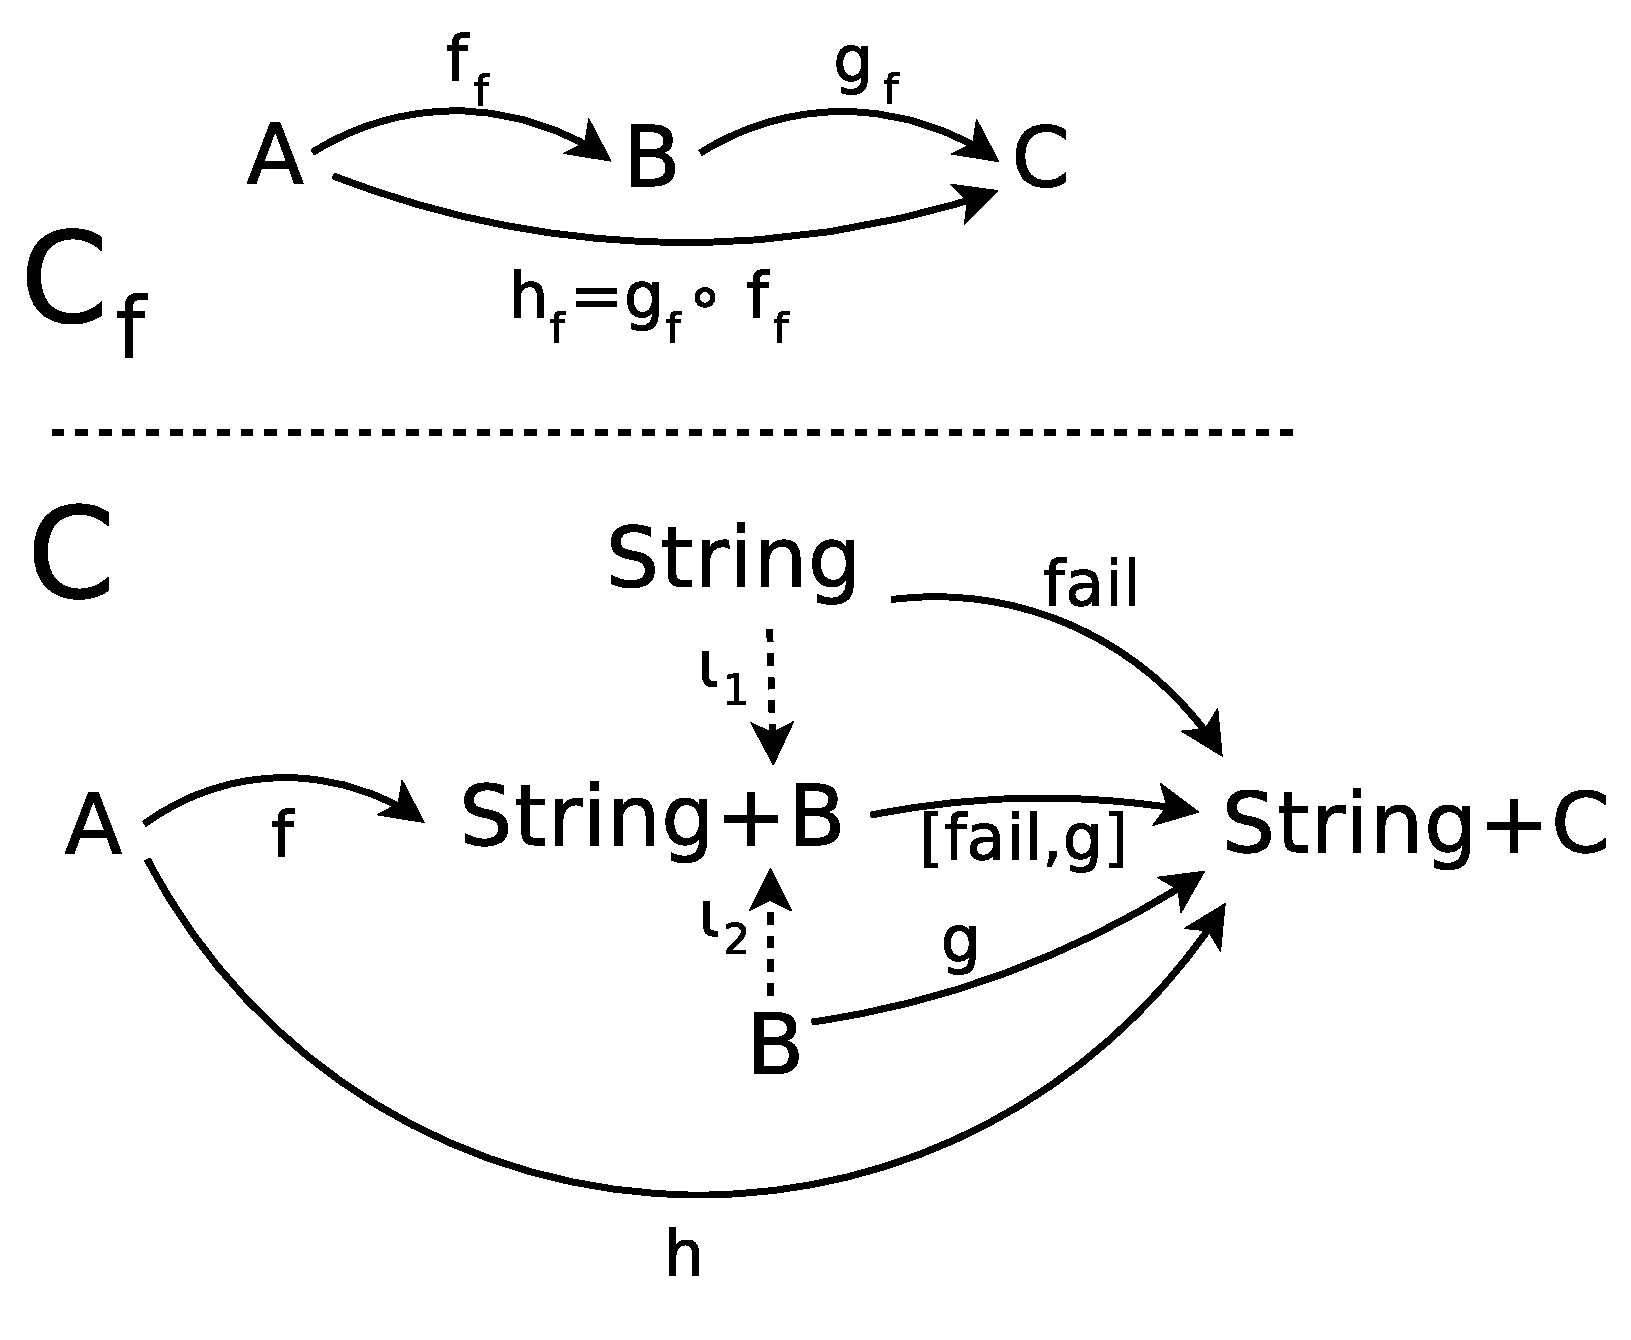
\includegraphics[scale=0.3]{images/cat_fail}
%     \caption{Komposition beim Fail-Funktor}
%   \end{figure}
% \end{frame}

% \begin{frame}{Der Funktor State}
%   \begin{itemize}
%   \item Nun sollen Zustände vom Typ S weitergereicht werden
%   \item Wieder verstecken, neue Kategorie $C_{s}$ mit Funktor
%     $State : C_{s} \rightarrow C$
%   \item $f_{s} : A \rightarrow B$ wird abgebildet auf
%     $f = A \times S \rightarrow B \times S$
%   \item Komposition in $C_{s}$ einfach
%     \begin{figure}
%       \centering
%       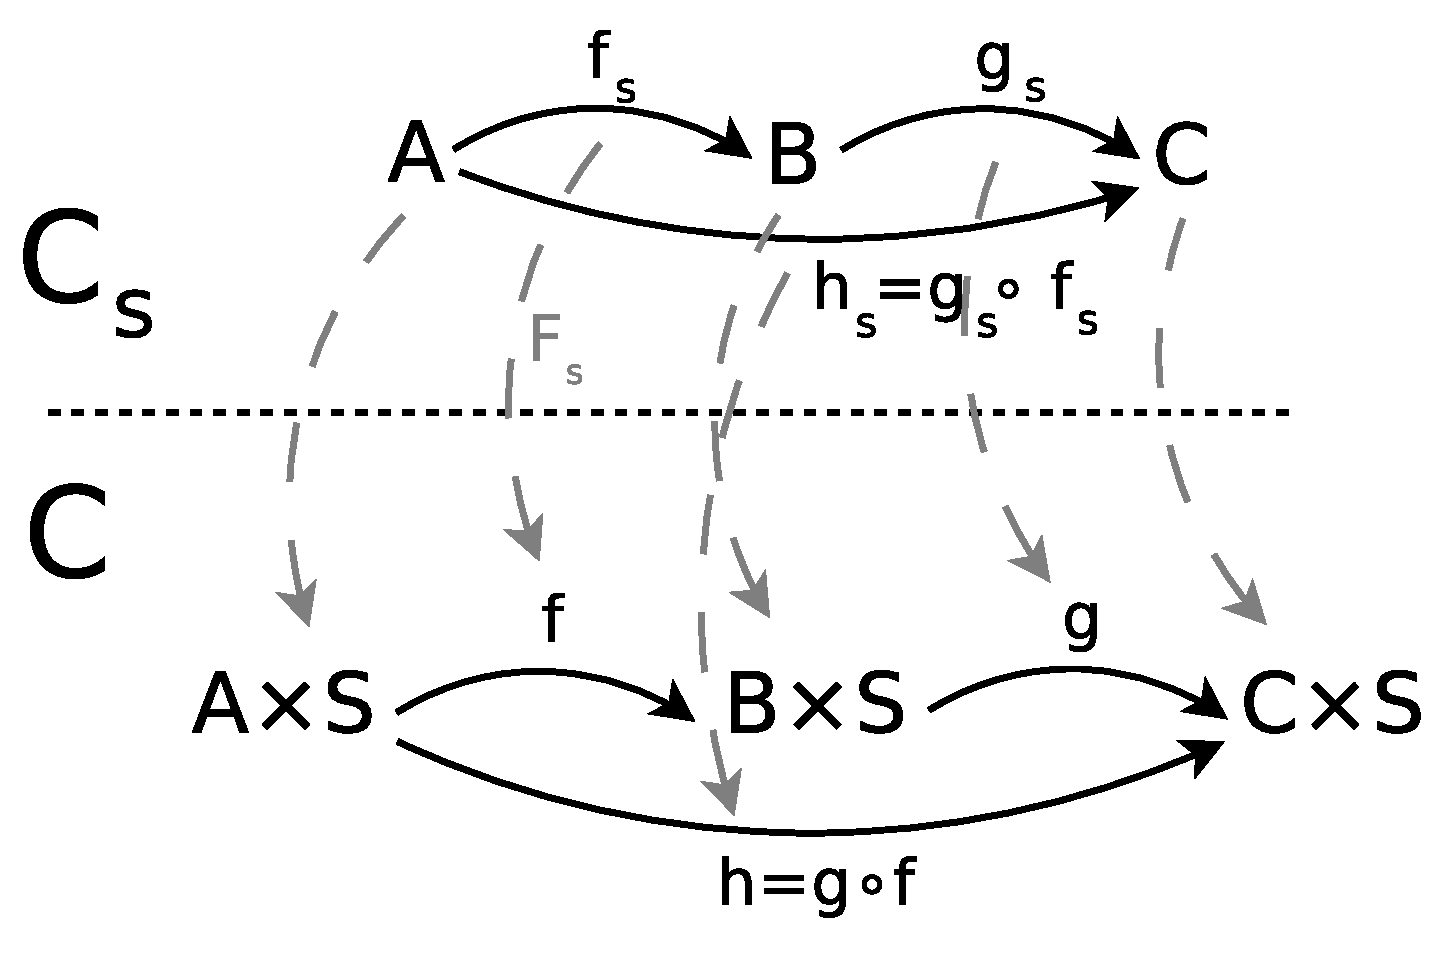
\includegraphics[scale=0.2]{images/cat_state}
%       \caption{Komposition beim State-Funktor}
%     \end{figure}
%   \end{itemize}
% \end{frame}

% \begin{frame}{Der Funktor State (2)}
%   \begin{itemize}
%   \item Etwas Tricky: Produkte in $C_{s}$
%   \item Arbeiten mit Zuständen: Lesen \& Schreiben:
%   \item Lesen: $get_s : \forall a : a \rightarrow S$
%   \item Schreiben: $put_s : S \rightarrow *$
%   \item Zum Parsen: $S = List$ $of$ $T$ mit Token-Typ $T$
%   \end{itemize}
% \end{frame}

% \begin{frame}{Der Parse-Funktor}
%   \begin{itemize}
%   \item Kombination von Fail und State zu einem Funktor Parse
%   \item $C_p = C_{ffs}$
%   \item Zwei Fail-Funktoren für bessere Fehlermeldungen
%   \item Beispiel:
%     \begin{itemize}
%     \item Grammatik: \texttt{\{.*\} $\bigvee$ [.*]}
%     \item Eingabewort: \texttt{\{ABC}
%     \item Schlecht: \texttt{"'Expected [, got \{"'}
%     \item Gut: \texttt{"'Expected \}, got end of stream"'}
%     \item Scheitern nach \texttt{\{} soll Backtracking aushebeln \\
%       $\Rightarrow$ \textit{innerer Fail}
%     \end{itemize}
%   \end{itemize}
% \end{frame}

% \begin{frame}{Der Parse-Funktor (2)}
%   \begin{itemize}
%   \item Flexible Parser-Anwendungen dank Funktor
%     \begin{itemize}
%     \item Funktionale Parser: $Hask_p$
%     \item Parser mit Side-Effects: $IO_p$
%     \item Parser mit anderen Extras: Weitere Funktoren möglich
%     \end{itemize}
%   \item Token-Typ Variabel:
%     \begin{itemize}
%     \item \texttt{Char} für Textdateien
%     \item \texttt{Bool} für Bytestreams
%     \item \texttt{Sexp} für S-Expressions
%     \end{itemize}
%   \item Parser-Bibliothek enthält dazu:
%     \begin{itemize}
%     \item Praktische Funktionen zum Parser-Erzeugen (Blick in \texttt{Parser.hs})
%     \item Möglichkeiten zum Aufruf von inneren Parsern
%     \item Konzepte zum Verschalten von Parsern und Compilern
%     \end{itemize}
%   \end{itemize}
% \end{frame}

% \begin{frame}{Parsen von S-Expressions}
%   \begin{itemize}
%   \item Besonderheit: Token können selbst Listen sein
%   \item Lösung: Als Stream behandeln, \texttt{compNode} wendet Parser
%     auf inneren Stream an
%     \begin{itemize}
%     \item Beispiel: Lesen von \texttt{(hallo welt)}
%     \item \texttt{compNode (symeq "'hallo"' >>> symeq "'welt"') } % <<
%     \end{itemize}
%   \item Makros: \texttt{compNode mit Prüfung des ersten Symbols}
%     \begin{itemize}
%     \item obiges Beispiel: \texttt{macro "'hallo"' (symeq "'welt"')}
%     \item Stimmt das erste Symbol überein, wird das Backtracking aufgehoben
%     \end{itemize}
%   \end{itemize}
% \end{frame}

\end{document}
